\documentclass{article}

%%% Fill details here (in the second brackets)
\newcommand{\name}{Hao Sun}     % Your name (First Last)
\newcommand{\wustlkey}{sun.hao}             % Your WUSTL Key
%%%



%%%%%%%%%%%%%%%%%%%%%% Formatting Stuff %%%%%%%%%%%%%%%%%%%%%%%%%%%
\usepackage{times}
\usepackage[T1]{fontenc}

\setlength{\parskip}{1em}\setlength{\parindent}{0pt}
\linespread{1.25}
\usepackage[margin=0.7in,top=1in]{geometry}\usepackage{fancyhdr}
\pagestyle{fancy}\lhead{\bf \name}\rhead{\bf \wustlkey}\cfoot{\thepage}
\newcommand{\info}{\clearpage \subsection*{Information}}

\newcommand{\solution}[1]{\clearpage \subsection*{Solution #1}}  % define a new command \solution without index number
\newcommand{\spart}[1]{\paragraph{(#1)}} 
%%%%%%%%%%%%%%%%%%%%%%%%%%%%%%%%%%%%%%%%%%%%%%%%%%%%%%%%%%%%%%%%%%%


%%% Add any more packages if you want to
\usepackage{amsmath,graphicx}


\begin{document}
%%%%% Main Body goes here

% Begin solution to every problem like this.
\solution{1}

\spart{a} 
Assume a point $P = [X,Y,Z,1]^T$ in 3D world, $P_1,P_2$ are corresponded points in images of camera1 and camera 2. $P_1 = [x,y,1]^T, P_2 = [x',y,1]^T$. So we have: 
\begin{align}
	P_1 \sim K[I|\bar{0}]P\\
	P_2 \sim K[I|t]P\\
	K = \left[
		\begin{array}{ccc}
		f & 0 & 0\\
		0 & f & 0\\
		0 & 0 & 1
		\end{array}
		\right]\\
	t = [-t_x,0,0]^T
\end{align}
The homogeneous coordinate of $P_1 and P_2$ are as following:
\begin{align}
	P_1 = \left[
			\begin{array}{c}
			Xf\\
			Yf\\
			Z
			\end{array}
		\right]
	P_2 = \left[
			\begin{array}{c}
			Xf - t_xf\\
			Yf\\
			Z
			\end{array}
		\right]
	\end{align}
We get $x = \frac{XF}{Z}$, $x' = \frac{Xf-t_xf}{Z}$. Therefore:
\begin{align}
	d = x - x' = \frac{XF}{Z} -  \frac{Xf-t_xf}{Z} = \frac{ft_x}{Z} 
\end{align}
\spart{b} 
Based on the equation $X\alpha+Y\beta+Z\gamma = k$(where $X=\frac{Zx}{f}, Y=\frac{Zy}{f}$, because $x=\frac{Xf}{Z}$ and $y=\frac{Yf}{Z}$ according to equation (5)), we can get the following equations:
 
\begin{align}
	rZ = k - \frac{x\alpha}{f}Z - \frac{y\beta}{f}Z \Rightarrow Z = \frac{k}{\gamma+\frac{x\alpha}{f} + \frac{y\beta}{f}}
\end{align}
Based on equation (6) and (7), $d = ax + by + c$ can be represented by:
\begin{align}
	d = \frac{t_x}{k}(x\alpha + y\beta + f\gamma)
\end{align}

\spart{c} 
The homogeneous coordinate of $P_1 and P_2$ are as following:
\begin{align}
	P_1 =  \left[
			\begin{array}{c}
			Xf\\
			Yf\\
			Z
			\end{array}
		\right]
	P_2 = \left[
			\begin{array}{c}
			Xf\\
			Yf\\
			Z-t_z
			\end{array}
		\right]
\end{align}
Therefore, we can get $x', y'$ as following:
\begin{align}
	x' = \frac{xZ}{Z-t_z} \\
	y' = \frac{yZ}{Z-t_z}
\end{align}
The set of possible $(x',y')$ that could match to $(x,y)$ is: 
\begin{align}
	\frac{x'}{y'} = \frac{x}{y} 
\end{align}

\solution{2}

\spart{a}
buildcv
\begin{figure*}[h!]
  \centering
	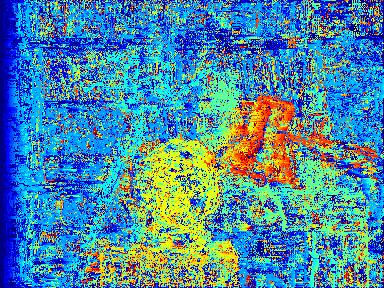
\includegraphics[height=24em]{code/outputs/prob2a.jpg}
	  \caption{Disparity Image by buildcv}
\end{figure*}

\spart{b}
bfilt
\begin{figure*}[h!]
  \centering
	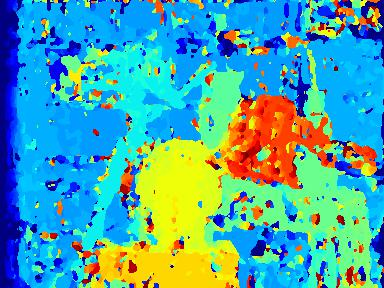
\includegraphics[height=24em]{code/outputs/prob2b.jpg}
	  \caption{Smoothed cost volume using Bilateral filtering}
\end{figure*}

\solution{3}
\spart{a}
viterbilr
\begin{figure*}[h!]
  \centering
	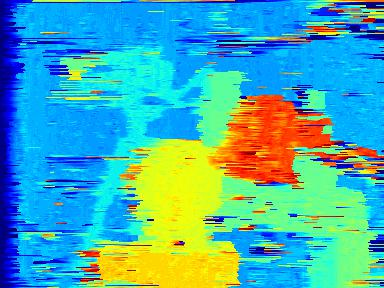
\includegraphics[height=24em]{code/outputs/prob3a.jpg}
	  \caption{Smoothed cost volume using forward-backward algorithm}
\end{figure*}

\spart{b}
SGM

\begin{figure*}[h!]
  \centering
	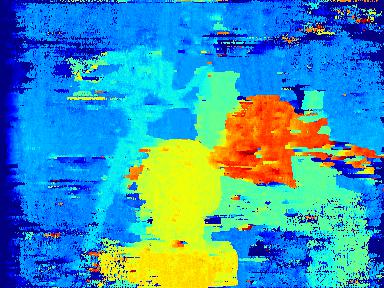
\includegraphics[height=24em]{code/outputs/prob3b.jpg}
	  \caption{Smoothed cost volume using SGM}
\end{figure*}

\solution{4}

\begin{figure*}[h!]
  \centering
	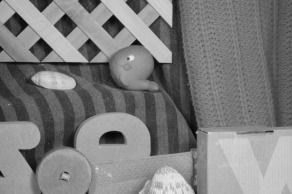
\includegraphics[height=15em]{code/inputs/frame10.jpg}
	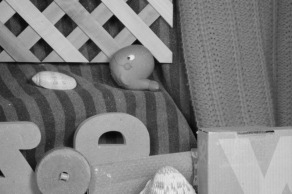
\includegraphics[height=15em]{code/inputs/frame11.jpg}
	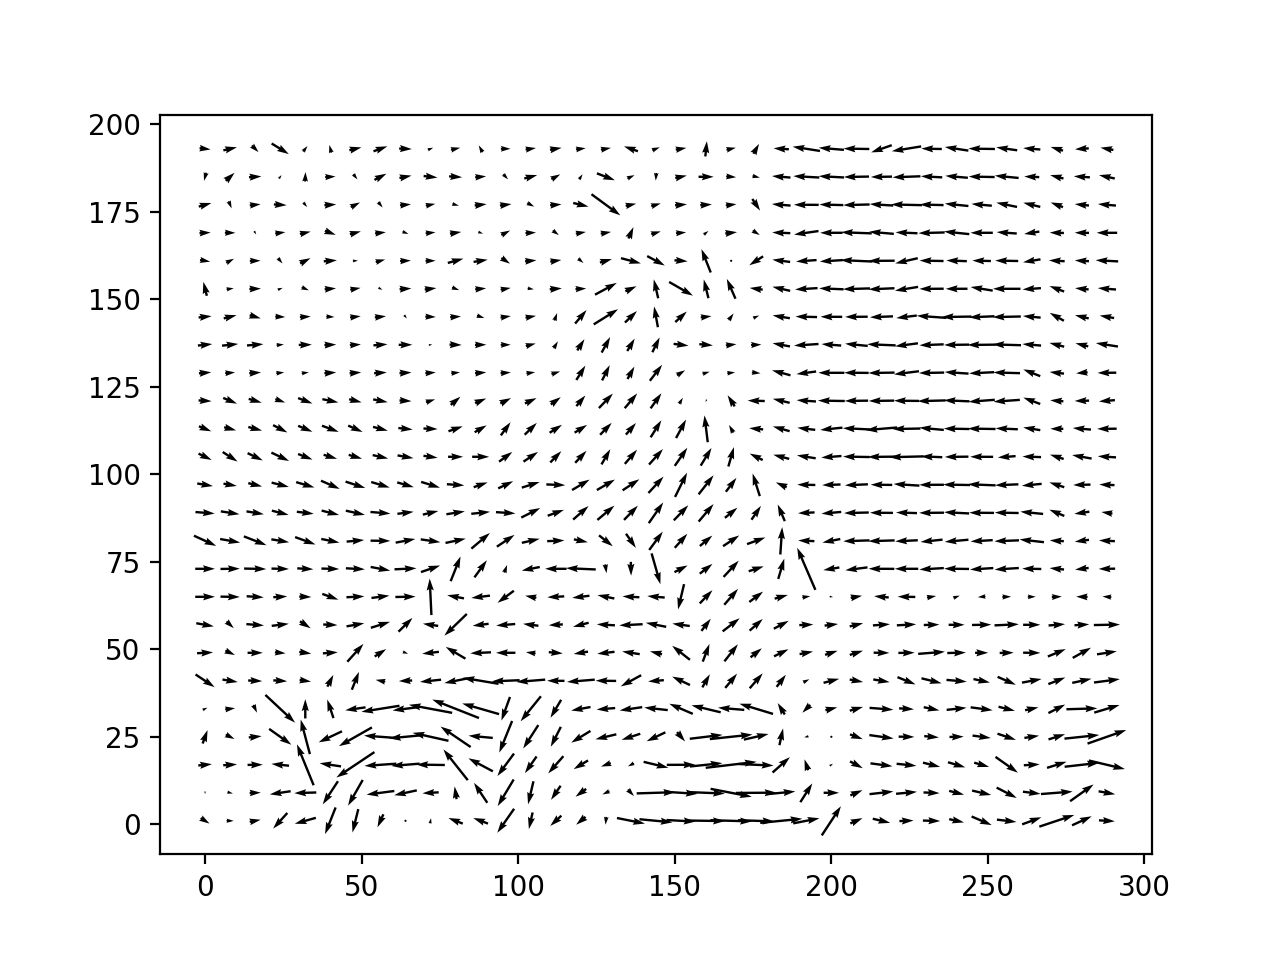
\includegraphics[height=30em]{code/outputs/prob4.png}
	  \caption{Optical Flow by Lucas Kanade Method}
\end{figure*}

\info

This problem set took approximately 30 hours of effort.

I discussed this problem set with:
\begin{itemize}
\item Sijia Wang
\item Chunyuan Li
\item Jiarui Xing
\end{itemize}

% Note that you might have to escape some special symbols in URLS like \_
I also got hints from the following sources:
\begin{itemize}
\item lecture ppts
\end{itemize}

\end{document}
